\chapter{CodeWarrior for MCU}

\section{Vedere de ansamblu asupra utilitarului}
Figura \ref{fig:CodeWarrior-VedereDeAnsamblu} ilustrează cele mai importante ferestre din mediul de dezvoltare \textit{CodeWarrior for MCU}. În partea de sus avem meniuri și butoane pentru acces rapid la anumite funcționalități, în stânga avem detalii legate de proiectele create și fișierele asociate lor, în centru ecranului apare un editor prin care se poate modifica conținutul fișierelor unui proiect, iar în partea de jos se poate observa dacă proiectul nostru conține erori.

\begin{figure}[h!]
  \vspace{-20pt}
  \center{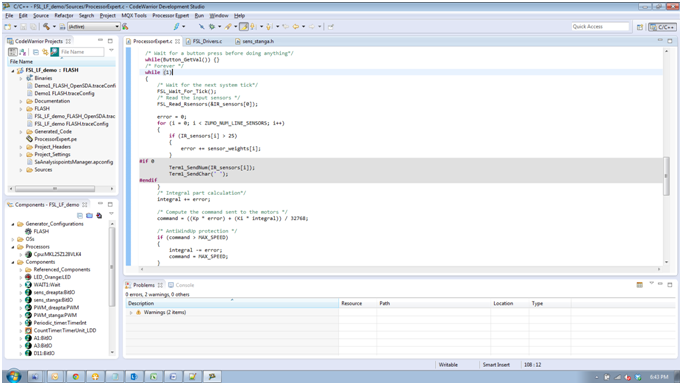
\includegraphics[width=1.0 \textwidth]{images/CodeWarriorMCU.png}}
  \vspace{-15pt}
  \caption{\label{fig:CodeWarrior-VedereDeAnsamblu} CodeWarrior for MCU - Vedere de ansamblu}
  \vspace{-20pt}
\end{figure}

\section{Compilarea proiectului}

\begin{wrapfigure}{r}{0.5\textwidth}
  \vspace{-20pt}
  \center{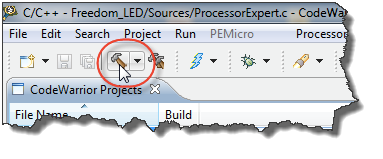
\includegraphics[width=0.5 \textwidth]{images/BuildProject.png}}
  \vspace{-10pt}
  \caption{\label{fig:CodeWarrior-CompilareProiect} Cum se poate compila proiectul}
  \vspace{-20pt}
\end{wrapfigure}

Pentru a compila proiectul, după ce în prealabil s-a generat codul folosind ProcessorExpert și voi v-ați scris codul vostru sursă, puteti folosi butonul din figura \ref{fig:CodeWarrior-CompilareProiect} sau de ce nu puteți folosi meniul principal și anume opțiunea \textit{Project $\rightarrow$ Build Project}. Indiferent de varianta aleasă rezultatul va fi același.